% To familiarize yourself with this template, the body contains
% some examples of its use.  Look them over.  Then you can
% run LaTeX on this file.  After you have LaTeXed this file then
% you can look over the result either by printing it out with
% dvips or using xdvi.
%

\documentclass[twoside,english]{article}
\setlength{\oddsidemargin}{0.25 in}
\setlength{\evensidemargin}{-0.25 in}
\setlength{\topmargin}{-0.6 in}
\setlength{\textwidth}{6.5 in}
\setlength{\textheight}{8.5 in}
\setlength{\headsep}{0.75 in}
\setlength{\parindent}{0 in}
\setlength{\parskip}{0.1 in}

%
% ADD PACKAGES here:
%

\usepackage{amsmath,amsfonts,graphicx,algorithm,caption}
\usepackage[noend]{algpseudocode}
\usepackage{hyperref}
\usepackage{natbib}
\usepackage[document]{ragged2e}
\usepackage{graphicx} %package to manage images
\usepackage{amsmath}
\usepackage{mathtools}
\usepackage{xcolor}

% The following commands set up the lecnum (lecture number)
% counter and make various numbering schemes work relative
% to the lecture number.
%
\newcounter{lecnum}
\renewcommand{\thepage}{\arabic{page}}
\renewcommand{\thesection}{\arabic{section}}
\renewcommand{\theequation}{\arabic{equation}}
\renewcommand{\thefigure}{\arabic{figure}}
\renewcommand{\thetable}{\arabic{table}}
\makeatletter
\def\BState{\State\hskip-\ALG@thistlm}
\makeatother
%
% The following macro is used to generate the header.
%
\newcommand{\lecture}[4]{
   \pagestyle{myheadings}
   \thispagestyle{plain}
   \newpage
   %\setcounter{lecnum}{#1}
   \setcounter{page}{1}
   \noindent
   \begin{center}
   \framebox{
      \vbox{\vspace{2mm}
    \hbox to 6.28in { {\bf IE 643: Deep Learning - Theory and Practice
		\hfill July-Dec 2026} }
       \vspace{4mm}
       \hbox to 6.28in { {\Large \hfill Project Report: #1  \hfill} }
       \vspace{2mm}
       \vspace{2mm}
       \hbox to 6.28in { {\it Team Name: #2 \hfill Team Members: #3} }
       %\vspace{2mm}}
       %\hbox to 6.28in { {\it Due Date: 01-August-2018} }
      \vspace{2mm}}
   }
   \end{center}
%   \markboth{Assignment #1: #2}{Assignment #1: #2}

   %{\bf Note}: {\it LaTeX template courtesy of UC Berkeley EECS dept.}

   %{\bf Disclaimer}: {\it These notes have not been subjected to the
   %usual scrutiny reserved for formal publications.  They may be distributed
   %outside this class only with the permission of the Instructor.}
   \vspace*{4mm}
}
%
% Convention for citations is authors' initials followed by the year.
% For example, to cite a paper by Leighton and Maggs you would type
% \cite{LM89}, and to cite a paper by Strassen you would type \cite{S69}.
% (To avoid bibliography problems, for now we redefine the \cite command.)
% Also commands that create a suitable format for the reference list.
\renewcommand{\cite}[1]{[#1]}
\def\beginrefs{\begin{list}%
        {[\arabic{equation}]}{\usecounter{equation}
         \setlength{\leftmargin}{2.0truecm}\setlength{\labelsep}{0.4truecm}%
         \setlength{\labelwidth}{1.6truecm}}}
\def\endrefs{\end{list}}
\def\bibentry#1{\item[\hbox{[#1]}]}

%Use this command for a figure; it puts a figure in wherever you want it.
%usage: \fig{NUMBER}{SPACE-IN-INCHES}{CAPTION}
\newcommand{\fig}[3]{
			\vspace{#2}
			\begin{center}
			Figure #1:~#3
			\end{center}
	}
% Use these for theorems, lemmas, proofs, etc.
\newtheorem{theorem}{Theorem}[lecnum]
\newtheorem{lemma}[theorem]{Lemma}
\newtheorem{proposition}[theorem]{Proposition}
\newtheorem{claim}[theorem]{Claim}
\newtheorem{corollary}[theorem]{Corollary}
\newtheorem{definition}[theorem]{Definition}
\newenvironment{proof}{{\bf Proof:}}{\hfill\rule{2mm}{2mm}}

% **** IF YOU WANT TO DEFINE ADDITIONAL MACROS FOR YOURSELF, PUT THEM HERE:
\newcommand{\R}{\mathbb{R}}

\begin{document}
%FILL IN THE RIGHT INFO.
%\lecture{**LECTURE-NUMBER**}{**DATE**}{**LECTURER**}{**SCRIBE**}
\lecture{Creating Graphics Programs from Images}{Your team's name}{Roll numbers of team members}
%\footnotetext{These notes are partially based on those of Nigel Mansell.}

% **** YOUR NOTES GO HERE:

% Some general latex examples and examples making use of the
% macros follow.  
%**** IN GENERAL, BE BRIEF. LONG SCRIBE NOTES, NO MATTER HOW WELL WRITTEN,
%**** ARE NEVER READ BY ANYBODY.

\begin{abstract}
	This project report contains the details on our project which aims to infer graphics software programs from hand-drawn images. We describe the deep learning tools involved in our project. In particular, we explain about the deep neural network architectures, the loss functions and activation functions used and the training algorithm used. We have tried a new deep learning architecture and superior results are presented using the proposed architecture.  
\end{abstract}

\section{Introduction}

Provide a short introduction about the project with proper motivation and applications. Give a broad overview of the project without getting much into the details. 

Explain the structure of the project report as below:

We provide a survey of existing literature in Section \ref{sec:litsurvey}. Our proposal for the project is described in Section \ref{sec:our_proj}. We give details on experiments in Section \ref{sec:exp}. A description of future work is given in Section \ref{sec:Plan for Novelty Assessment}. We conclude with a short summary and pointers to forthcoming work in Section \ref{sec:conclusion}.

\section{Project Workflow}  
Outline the entire workflow of the project, beginning with the problem statement and detailing how the team has advanced towards completing the task. This section should utilize concise bullet points, and a workflow diagram would be appreciated.


\section{Literature Survey} \label{sec:litsurvey}
This section should include all relevant work, papers, and approaches that the team has reviewed in order to achieve the task.

Example:

Our project draws inspiration from a closely related work by Ellis et al. \citep{paper}. In their paper \citep{paper}, the authors describe a three-step process where an input hand-drawn image is first used to generate a program specification (spec) which is then used to generate a graphics software program which is later rendered to generate the hand-drawn image as a graphics object (like a bitmap image, jpeg image, etc.).  This process is illustrated in Figure \ref{threestepprocimg}.

\begin{figure}[!h]
	\centering
	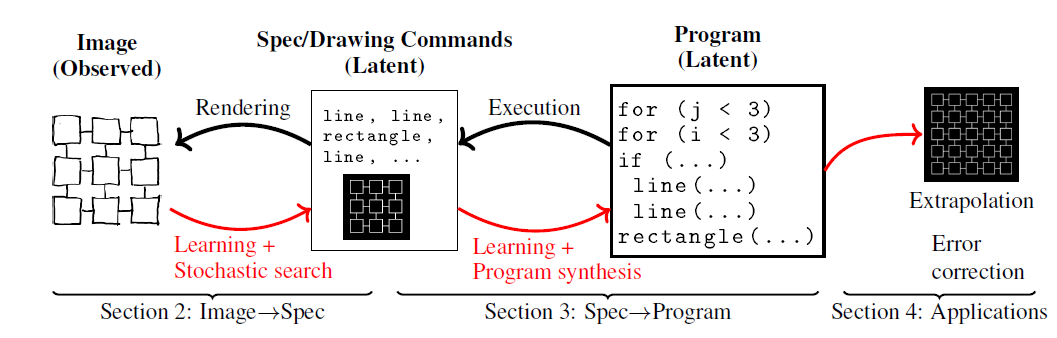
\includegraphics[scale=0.8]{threestepprocess}
	\caption{Three Step Process to generate program specs from image and then to convert specs to graphics programs and later render the programs to graphics objects}\label{threestepprocimg}
\end{figure}


The neural network structure consists of two major components one of which is used to infer program specifications (\textbf{specs}) from the input image, and the other network to generate graphics programs to specs. 


The neural network to infer spec $S$ from an input image $I$ uses ideas from Neurally guided procedural models \citep{paper2} and attend-infer-repeat \citep{paper3} models. The network is trained on sampled specs $S$ and target images $I$ from randomly generated scenes. The network is trained by maximizing the parametrized likelihood $P_\theta(S|I)$ of inferring a spec $S$ given an image $I$, with the parameters $\theta$ being the parameters associated with the neural network. The network structure is illustrated in Figure \ref{specgenimg}. For further robustness to correct the network errors, the network outputs are further processed by a sequential Monte Carlo sampling scheme \citep{book1}.    
  
\begin{figure}[!h]
	\centering
	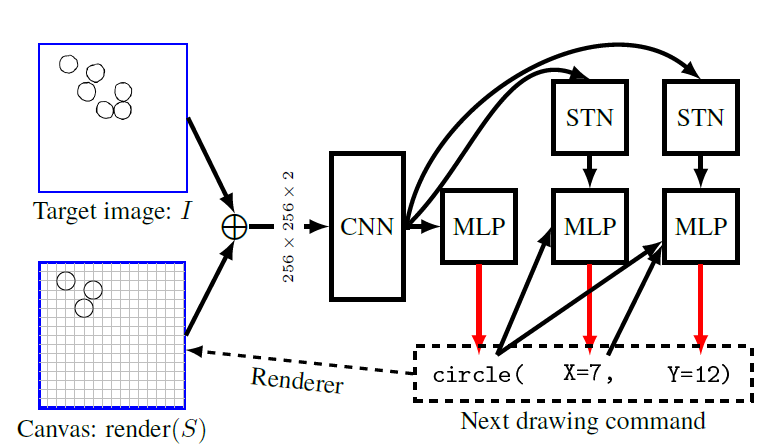
\includegraphics[scale=0.8]{specgen}
	\caption{Neural architecture to infer specs from images.}\label{specgenimg}
\end{figure}


Though the specs capture the contents of a scene, they do not contain information about repeated motifs or symmetries. To capture these high-level features, graphics programs (typically software programs) are synthesized from specs. The grammar used in the synthesis of graphics program is restricted to a set of grammar rules given in Figure \ref{grammarimg}.


\begin{figure}[!h]
	\centering
	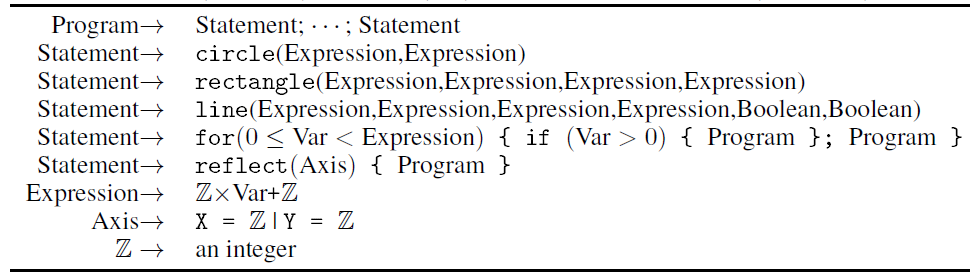
\includegraphics[scale=0.8]{grammar}
	\caption{Grammar rules used for graphics program.}\label{grammarimg}
\end{figure}
 
 The best graphics program that satisfies the grammar rules listed in Figure \ref{grammarimg} is synthesized so that it best captures the spec. The closeness of a synthesized program $p$ with the spec $S$ is captured by an indicator function ${\mathbb{I}}(p \text{is consistent with } S)$. In addition the cost of a program $p$ (denoted by $\text{cost}(p)$) is measured using the number of program statements in $p$. Thus the next network seeks to find the minimum cost program which is consistent with the program rules in Figure \ref{grammarimg}. Thus the following objective is used: 
 \begin{align}
 \text{PROG}(S) = \arg\max_{p \text{ obeys Grammar}} {\mathbb{I}}(p \text{is consistent with } S) \exp(-\text{cost}(p)). \label{synthesis_obj}
 \end{align}
  To measure this consistency of a program $p$ with a spec $S$, a Sketch tool \citep{thesis1} is used. Sketch tool transforms the consistency check condition to a constraint satisfaction problem and uses a SAT solver to find a min-cost program satisfying the spec. 
  
 A few experiments on a dataset are provided which indicate the usefulness of the approach.


\section{Proposed Approach or Approaches} \label{sec:our_proj}

Give details on the proposed approach or approaches, which team has tried. Explain how it is different from existing work. Explain all the neural network structure to be used. Explain all other required details.

\subsection{Work done before prep-presentation review} 
This section can be populated from your prep-presentation project report. 

\subsection{Work done after prep-presentation review} 

Give details on the work done after the prep-presentation project review. Explain how it is significant. Explain all the neural network structures used. Explain all other required details.

\section{Data set Details} \label{sec:data}

Explain all details  on the data sets used for the project. Description of data size and attributes, nature and type of data (image/audio/text/video etc.), data pre-processing techniques used should be illustrated. Other relevant details on data procurement (the website from where the data is obtained), and how the data is to be used in experiments should be described. 

\section{Experiments} \label{sec:exp}

\textcolor{red}{The team should include all experiments, even those with negative results, and address all experiments that were performed.}


Give details on experiments performed. Training procedure and algorithm, the settings used for optimization algorithm and other relevant algorithmic details need to be included. Details on the hardware configuration should also be described. 


\section{Results}\label{sec:results}

Add suitable plots and tables describing the results obtained during the project. Comparative results should be included if new ideas are tried. Description of the results and the inferences made using the results should be described. 

\section{Plan for Novelty Assessment} \label{sec:Plan for Novelty Assessment}

Explain the work to be done further for Novelty Assessment. 

\section{Conclusion} \label{sec:conclusion}

Conclude by giving a summary of your project, summarizing the problem, the methods used, and the significance of results obtained. Give some indications of future work to be done. 

\bibliographystyle{plain}
\bibliography{demo} % Because the file name is demo.bib


\end{document}

